% Created by tikzDevice version 0.10.1 on 2020-02-15 16:15:47
% !TEX encoding = UTF-8 Unicode
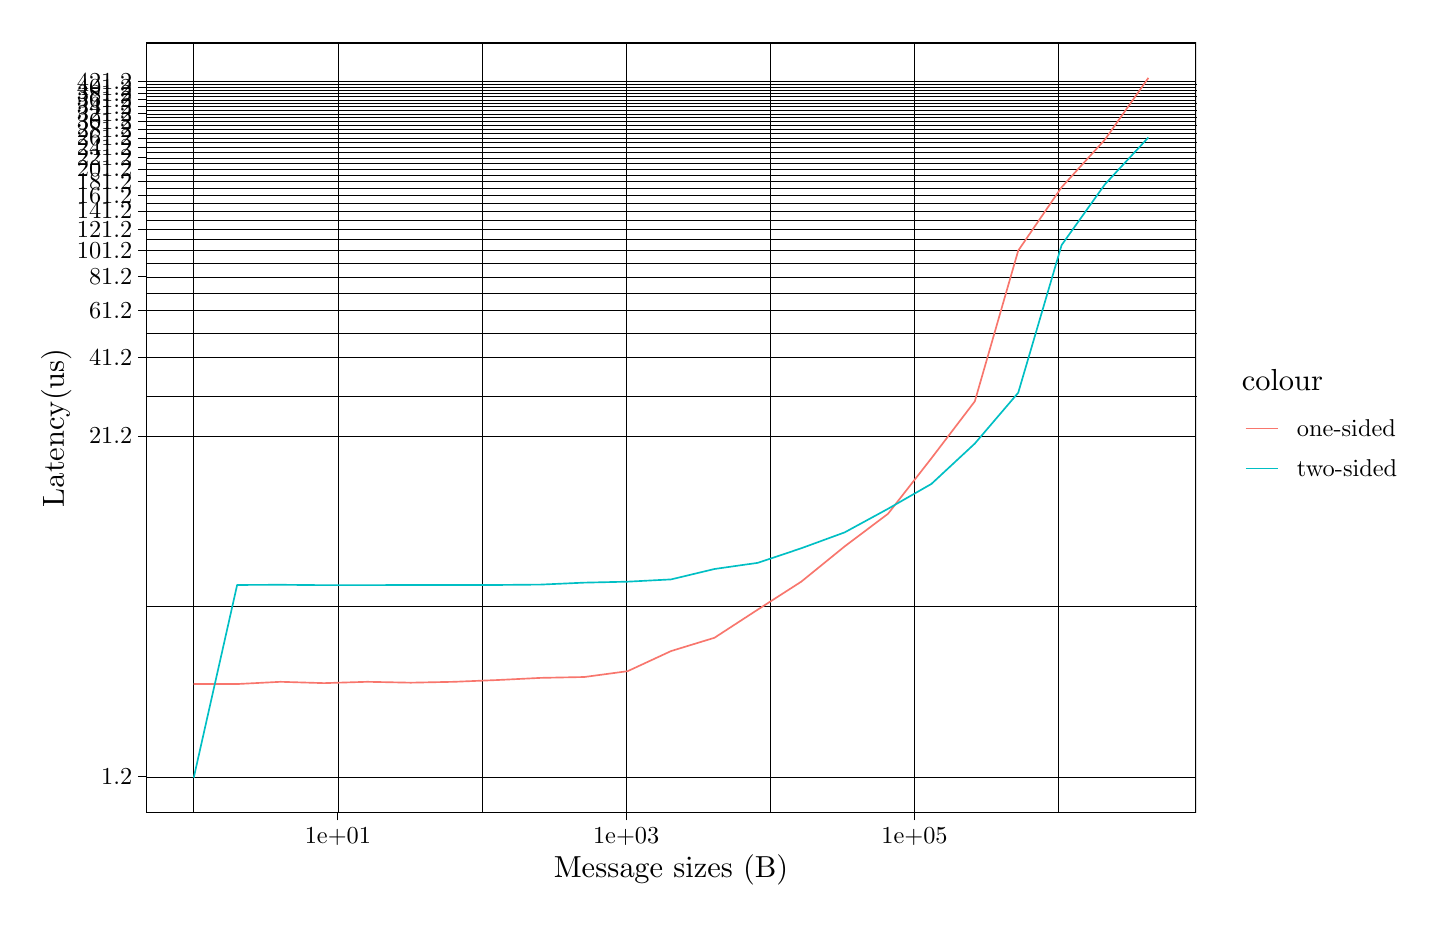
\begin{tikzpicture}[x=1pt,y=1pt]
\definecolor{fillColor}{RGB}{255,255,255}
\path[use as bounding box,fill=fillColor,fill opacity=0.00] (0,0) rectangle (505.89,314.37);
\begin{scope}
\path[clip] (  0.00,  0.00) rectangle (505.89,314.37);
\definecolor{drawColor}{RGB}{255,255,255}
\definecolor{fillColor}{RGB}{255,255,255}

\path[draw=drawColor,line width= 0.6pt,line join=round,line cap=round,fill=fillColor] (  0.00,  0.00) rectangle (505.89,314.37);
\end{scope}
\begin{scope}
\path[clip] ( 42.76, 30.72) rectangle (422.22,308.87);
\definecolor{fillColor}{RGB}{255,255,255}

\path[fill=fillColor] ( 42.76, 30.72) rectangle (422.22,308.87);
\definecolor{drawColor}{RGB}{0,0,0}

\path[draw=drawColor,line width= 0.0pt,line join=round] ( 42.76,105.27) --
	(422.22,105.27);

\path[draw=drawColor,line width= 0.0pt,line join=round] ( 42.76,181.04) --
	(422.22,181.04);

\path[draw=drawColor,line width= 0.0pt,line join=round] ( 42.76,203.76) --
	(422.22,203.76);

\path[draw=drawColor,line width= 0.0pt,line join=round] ( 42.76,218.30) --
	(422.22,218.30);

\path[draw=drawColor,line width= 0.0pt,line join=round] ( 42.76,229.08) --
	(422.22,229.08);

\path[draw=drawColor,line width= 0.0pt,line join=round] ( 42.76,237.66) --
	(422.22,237.66);

\path[draw=drawColor,line width= 0.0pt,line join=round] ( 42.76,244.80) --
	(422.22,244.80);

\path[draw=drawColor,line width= 0.0pt,line join=round] ( 42.76,250.91) --
	(422.22,250.91);

\path[draw=drawColor,line width= 0.0pt,line join=round] ( 42.76,256.26) --
	(422.22,256.26);

\path[draw=drawColor,line width= 0.0pt,line join=round] ( 42.76,261.01) --
	(422.22,261.01);

\path[draw=drawColor,line width= 0.0pt,line join=round] ( 42.76,265.28) --
	(422.22,265.28);

\path[draw=drawColor,line width= 0.0pt,line join=round] ( 42.76,269.17) --
	(422.22,269.17);

\path[draw=drawColor,line width= 0.0pt,line join=round] ( 42.76,272.73) --
	(422.22,272.73);

\path[draw=drawColor,line width= 0.0pt,line join=round] ( 42.76,276.02) --
	(422.22,276.02);

\path[draw=drawColor,line width= 0.0pt,line join=round] ( 42.76,279.07) --
	(422.22,279.07);

\path[draw=drawColor,line width= 0.0pt,line join=round] ( 42.76,281.92) --
	(422.22,281.92);

\path[draw=drawColor,line width= 0.0pt,line join=round] ( 42.76,284.60) --
	(422.22,284.60);

\path[draw=drawColor,line width= 0.0pt,line join=round] ( 42.76,287.11) --
	(422.22,287.11);

\path[draw=drawColor,line width= 0.0pt,line join=round] ( 42.76,289.49) --
	(422.22,289.49);

\path[draw=drawColor,line width= 0.0pt,line join=round] ( 42.76,291.74) --
	(422.22,291.74);

\path[draw=drawColor,line width= 0.0pt,line join=round] ( 42.76,293.88) --
	(422.22,293.88);

\path[draw=drawColor,line width= 0.0pt,line join=round] ( 60.01, 30.72) --
	( 60.01,308.87);

\path[draw=drawColor,line width= 0.0pt,line join=round] (164.18, 30.72) --
	(164.18,308.87);

\path[draw=drawColor,line width= 0.0pt,line join=round] (268.36, 30.72) --
	(268.36,308.87);

\path[draw=drawColor,line width= 0.0pt,line join=round] (372.54, 30.72) --
	(372.54,308.87);

\path[draw=drawColor,line width= 0.1pt,line join=round] ( 42.76, 43.73) --
	(422.22, 43.73);

\path[draw=drawColor,line width= 0.1pt,line join=round] ( 42.76,166.81) --
	(422.22,166.81);

\path[draw=drawColor,line width= 0.1pt,line join=round] ( 42.76,195.28) --
	(422.22,195.28);

\path[draw=drawColor,line width= 0.1pt,line join=round] ( 42.76,212.24) --
	(422.22,212.24);

\path[draw=drawColor,line width= 0.1pt,line join=round] ( 42.76,224.36) --
	(422.22,224.36);

\path[draw=drawColor,line width= 0.1pt,line join=round] ( 42.76,233.80) --
	(422.22,233.80);

\path[draw=drawColor,line width= 0.1pt,line join=round] ( 42.76,241.53) --
	(422.22,241.53);

\path[draw=drawColor,line width= 0.1pt,line join=round] ( 42.76,248.08) --
	(422.22,248.08);

\path[draw=drawColor,line width= 0.1pt,line join=round] ( 42.76,253.75) --
	(422.22,253.75);

\path[draw=drawColor,line width= 0.1pt,line join=round] ( 42.76,258.77) --
	(422.22,258.77);

\path[draw=drawColor,line width= 0.1pt,line join=round] ( 42.76,263.25) --
	(422.22,263.25);

\path[draw=drawColor,line width= 0.1pt,line join=round] ( 42.76,267.31) --
	(422.22,267.31);

\path[draw=drawColor,line width= 0.1pt,line join=round] ( 42.76,271.02) --
	(422.22,271.02);

\path[draw=drawColor,line width= 0.1pt,line join=round] ( 42.76,274.44) --
	(422.22,274.44);

\path[draw=drawColor,line width= 0.1pt,line join=round] ( 42.76,277.60) --
	(422.22,277.60);

\path[draw=drawColor,line width= 0.1pt,line join=round] ( 42.76,280.55) --
	(422.22,280.55);

\path[draw=drawColor,line width= 0.1pt,line join=round] ( 42.76,283.30) --
	(422.22,283.30);

\path[draw=drawColor,line width= 0.1pt,line join=round] ( 42.76,285.89) --
	(422.22,285.89);

\path[draw=drawColor,line width= 0.1pt,line join=round] ( 42.76,288.33) --
	(422.22,288.33);

\path[draw=drawColor,line width= 0.1pt,line join=round] ( 42.76,290.64) --
	(422.22,290.64);

\path[draw=drawColor,line width= 0.1pt,line join=round] ( 42.76,292.83) --
	(422.22,292.83);

\path[draw=drawColor,line width= 0.1pt,line join=round] ( 42.76,294.92) --
	(422.22,294.92);

\path[draw=drawColor,line width= 0.1pt,line join=round] (112.10, 30.72) --
	(112.10,308.87);

\path[draw=drawColor,line width= 0.1pt,line join=round] (216.27, 30.72) --
	(216.27,308.87);

\path[draw=drawColor,line width= 0.1pt,line join=round] (320.45, 30.72) --
	(320.45,308.87);
\definecolor{drawColor}{RGB}{248,118,109}

\path[draw=drawColor,line width= 0.6pt,line join=round] ( 60.01, 77.19) --
	( 75.69, 77.19) --
	( 91.37, 78.00) --
	(107.05, 77.52) --
	(122.73, 78.00) --
	(138.41, 77.68) --
	(154.09, 78.00) --
	(169.77, 78.64) --
	(185.45, 79.42) --
	(201.13, 79.73) --
	(216.81, 81.84) --
	(232.49, 89.11) --
	(248.17, 93.91) --
	(263.85,104.11) --
	(279.53,114.18) --
	(295.21,126.92) --
	(310.89,138.72) --
	(326.57,158.78) --
	(342.25,179.35) --
	(357.93,233.81) --
	(373.61,256.71) --
	(389.29,273.96) --
	(404.97,296.23);
\definecolor{drawColor}{RGB}{0,191,196}

\path[draw=drawColor,line width= 0.6pt,line join=round] ( 60.01, 43.37) --
	( 75.69,112.99) --
	( 91.37,113.06) --
	(107.05,112.92) --
	(122.73,112.92) --
	(138.41,112.99) --
	(154.09,112.99) --
	(169.77,112.99) --
	(185.45,113.13) --
	(201.13,113.83) --
	(216.81,114.18) --
	(232.49,115.00) --
	(248.17,118.76) --
	(263.85,120.99) --
	(279.53,126.25) --
	(295.21,131.99) --
	(310.89,140.52) --
	(326.57,149.51) --
	(342.25,164.09) --
	(357.93,182.45) --
	(373.61,235.81) --
	(389.29,257.80) --
	(404.97,274.70);
\definecolor{drawColor}{RGB}{0,0,0}

\path[draw=drawColor,line width= 0.6pt,line join=round,line cap=round] ( 42.76, 30.72) rectangle (422.22,308.87);
\end{scope}
\begin{scope}
\path[clip] (  0.00,  0.00) rectangle (505.89,314.37);
\definecolor{drawColor}{RGB}{0,0,0}

\node[text=drawColor,anchor=base west,inner sep=0pt, outer sep=0pt, scale=  0.88] at ( 26.57, 40.90) {1.2};

\node[text=drawColor,anchor=base west,inner sep=0pt, outer sep=0pt, scale=  0.88] at ( 22.17,163.98) {21.2};

\node[text=drawColor,anchor=base west,inner sep=0pt, outer sep=0pt, scale=  0.88] at ( 22.17,192.46) {41.2};

\node[text=drawColor,anchor=base west,inner sep=0pt, outer sep=0pt, scale=  0.88] at ( 22.17,209.42) {61.2};

\node[text=drawColor,anchor=base west,inner sep=0pt, outer sep=0pt, scale=  0.88] at ( 22.17,221.54) {81.2};

\node[text=drawColor,anchor=base west,inner sep=0pt, outer sep=0pt, scale=  0.88] at ( 17.77,230.98) {101.2};

\node[text=drawColor,anchor=base west,inner sep=0pt, outer sep=0pt, scale=  0.88] at ( 17.77,238.71) {121.2};

\node[text=drawColor,anchor=base west,inner sep=0pt, outer sep=0pt, scale=  0.88] at ( 17.77,245.25) {141.2};

\node[text=drawColor,anchor=base west,inner sep=0pt, outer sep=0pt, scale=  0.88] at ( 17.77,250.93) {161.2};

\node[text=drawColor,anchor=base west,inner sep=0pt, outer sep=0pt, scale=  0.88] at ( 17.77,255.94) {181.2};

\node[text=drawColor,anchor=base west,inner sep=0pt, outer sep=0pt, scale=  0.88] at ( 17.77,260.43) {201.2};

\node[text=drawColor,anchor=base west,inner sep=0pt, outer sep=0pt, scale=  0.88] at ( 17.77,264.49) {221.2};

\node[text=drawColor,anchor=base west,inner sep=0pt, outer sep=0pt, scale=  0.88] at ( 17.77,268.20) {241.2};

\node[text=drawColor,anchor=base west,inner sep=0pt, outer sep=0pt, scale=  0.88] at ( 17.77,271.62) {261.2};

\node[text=drawColor,anchor=base west,inner sep=0pt, outer sep=0pt, scale=  0.88] at ( 17.77,274.78) {281.2};

\node[text=drawColor,anchor=base west,inner sep=0pt, outer sep=0pt, scale=  0.88] at ( 17.77,277.72) {301.2};

\node[text=drawColor,anchor=base west,inner sep=0pt, outer sep=0pt, scale=  0.88] at ( 17.77,280.48) {321.2};

\node[text=drawColor,anchor=base west,inner sep=0pt, outer sep=0pt, scale=  0.88] at ( 17.77,283.07) {341.2};

\node[text=drawColor,anchor=base west,inner sep=0pt, outer sep=0pt, scale=  0.88] at ( 17.77,285.51) {361.2};

\node[text=drawColor,anchor=base west,inner sep=0pt, outer sep=0pt, scale=  0.88] at ( 17.77,287.82) {381.2};

\node[text=drawColor,anchor=base west,inner sep=0pt, outer sep=0pt, scale=  0.88] at ( 17.77,290.01) {401.2};

\node[text=drawColor,anchor=base west,inner sep=0pt, outer sep=0pt, scale=  0.88] at ( 17.77,292.09) {421.2};
\end{scope}
\begin{scope}
\path[clip] (  0.00,  0.00) rectangle (505.89,314.37);
\definecolor{drawColor}{RGB}{0,0,0}

\path[draw=drawColor,line width= 0.3pt,line join=round] ( 40.01, 43.73) --
	( 42.76, 43.73);

\path[draw=drawColor,line width= 0.3pt,line join=round] ( 40.01,166.81) --
	( 42.76,166.81);

\path[draw=drawColor,line width= 0.3pt,line join=round] ( 40.01,195.28) --
	( 42.76,195.28);

\path[draw=drawColor,line width= 0.3pt,line join=round] ( 40.01,212.24) --
	( 42.76,212.24);

\path[draw=drawColor,line width= 0.3pt,line join=round] ( 40.01,224.36) --
	( 42.76,224.36);

\path[draw=drawColor,line width= 0.3pt,line join=round] ( 40.01,233.80) --
	( 42.76,233.80);

\path[draw=drawColor,line width= 0.3pt,line join=round] ( 40.01,241.53) --
	( 42.76,241.53);

\path[draw=drawColor,line width= 0.3pt,line join=round] ( 40.01,248.08) --
	( 42.76,248.08);

\path[draw=drawColor,line width= 0.3pt,line join=round] ( 40.01,253.75) --
	( 42.76,253.75);

\path[draw=drawColor,line width= 0.3pt,line join=round] ( 40.01,258.77) --
	( 42.76,258.77);

\path[draw=drawColor,line width= 0.3pt,line join=round] ( 40.01,263.25) --
	( 42.76,263.25);

\path[draw=drawColor,line width= 0.3pt,line join=round] ( 40.01,267.31) --
	( 42.76,267.31);

\path[draw=drawColor,line width= 0.3pt,line join=round] ( 40.01,271.02) --
	( 42.76,271.02);

\path[draw=drawColor,line width= 0.3pt,line join=round] ( 40.01,274.44) --
	( 42.76,274.44);

\path[draw=drawColor,line width= 0.3pt,line join=round] ( 40.01,277.60) --
	( 42.76,277.60);

\path[draw=drawColor,line width= 0.3pt,line join=round] ( 40.01,280.55) --
	( 42.76,280.55);

\path[draw=drawColor,line width= 0.3pt,line join=round] ( 40.01,283.30) --
	( 42.76,283.30);

\path[draw=drawColor,line width= 0.3pt,line join=round] ( 40.01,285.89) --
	( 42.76,285.89);

\path[draw=drawColor,line width= 0.3pt,line join=round] ( 40.01,288.33) --
	( 42.76,288.33);

\path[draw=drawColor,line width= 0.3pt,line join=round] ( 40.01,290.64) --
	( 42.76,290.64);

\path[draw=drawColor,line width= 0.3pt,line join=round] ( 40.01,292.83) --
	( 42.76,292.83);

\path[draw=drawColor,line width= 0.3pt,line join=round] ( 40.01,294.92) --
	( 42.76,294.92);
\end{scope}
\begin{scope}
\path[clip] (  0.00,  0.00) rectangle (505.89,314.37);
\definecolor{drawColor}{RGB}{0,0,0}

\path[draw=drawColor,line width= 0.3pt,line join=round] (112.10, 27.97) --
	(112.10, 30.72);

\path[draw=drawColor,line width= 0.3pt,line join=round] (216.27, 27.97) --
	(216.27, 30.72);

\path[draw=drawColor,line width= 0.3pt,line join=round] (320.45, 27.97) --
	(320.45, 30.72);
\end{scope}
\begin{scope}
\path[clip] (  0.00,  0.00) rectangle (505.89,314.37);
\definecolor{drawColor}{RGB}{0,0,0}

\node[text=drawColor,anchor=base,inner sep=0pt, outer sep=0pt, scale=  0.88] at (112.10, 19.71) {1e+01};

\node[text=drawColor,anchor=base,inner sep=0pt, outer sep=0pt, scale=  0.88] at (216.27, 19.71) {1e+03};

\node[text=drawColor,anchor=base,inner sep=0pt, outer sep=0pt, scale=  0.88] at (320.45, 19.71) {1e+05};
\end{scope}
\begin{scope}
\path[clip] (  0.00,  0.00) rectangle (505.89,314.37);
\definecolor{drawColor}{RGB}{0,0,0}

\node[text=drawColor,anchor=base,inner sep=0pt, outer sep=0pt, scale=  1.10] at (232.49,  7.44) {Message sizes (B)};
\end{scope}
\begin{scope}
\path[clip] (  0.00,  0.00) rectangle (505.89,314.37);
\definecolor{drawColor}{RGB}{0,0,0}

\node[text=drawColor,rotate= 90.00,anchor=base,inner sep=0pt, outer sep=0pt, scale=  1.10] at ( 13.08,169.80) {Latency(us)};
\end{scope}
\begin{scope}
\path[clip] (  0.00,  0.00) rectangle (505.89,314.37);
\definecolor{fillColor}{RGB}{255,255,255}

\path[fill=fillColor] (433.22,142.34) rectangle (500.39,197.26);
\end{scope}
\begin{scope}
\path[clip] (  0.00,  0.00) rectangle (505.89,314.37);
\definecolor{drawColor}{RGB}{0,0,0}

\node[text=drawColor,anchor=base west,inner sep=0pt, outer sep=0pt, scale=  1.10] at (438.72,183.22) {colour};
\end{scope}
\begin{scope}
\path[clip] (  0.00,  0.00) rectangle (505.89,314.37);
\definecolor{fillColor}{RGB}{255,255,255}

\path[fill=fillColor] (438.72,162.29) rectangle (453.17,176.74);
\end{scope}
\begin{scope}
\path[clip] (  0.00,  0.00) rectangle (505.89,314.37);
\definecolor{drawColor}{RGB}{248,118,109}

\path[draw=drawColor,line width= 0.6pt,line join=round] (440.16,169.52) -- (451.73,169.52);
\end{scope}
\begin{scope}
\path[clip] (  0.00,  0.00) rectangle (505.89,314.37);
\definecolor{drawColor}{RGB}{248,118,109}

\path[draw=drawColor,line width= 0.6pt,line join=round] (440.16,169.52) -- (451.73,169.52);
\end{scope}
\begin{scope}
\path[clip] (  0.00,  0.00) rectangle (505.89,314.37);
\definecolor{fillColor}{RGB}{255,255,255}

\path[fill=fillColor] (438.72,147.84) rectangle (453.17,162.29);
\end{scope}
\begin{scope}
\path[clip] (  0.00,  0.00) rectangle (505.89,314.37);
\definecolor{drawColor}{RGB}{0,191,196}

\path[draw=drawColor,line width= 0.6pt,line join=round] (440.16,155.06) -- (451.73,155.06);
\end{scope}
\begin{scope}
\path[clip] (  0.00,  0.00) rectangle (505.89,314.37);
\definecolor{drawColor}{RGB}{0,191,196}

\path[draw=drawColor,line width= 0.6pt,line join=round] (440.16,155.06) -- (451.73,155.06);
\end{scope}
\begin{scope}
\path[clip] (  0.00,  0.00) rectangle (505.89,314.37);
\definecolor{drawColor}{RGB}{0,0,0}

\node[text=drawColor,anchor=base west,inner sep=0pt, outer sep=0pt, scale=  0.88] at (458.67,166.49) {one-sided};
\end{scope}
\begin{scope}
\path[clip] (  0.00,  0.00) rectangle (505.89,314.37);
\definecolor{drawColor}{RGB}{0,0,0}

\node[text=drawColor,anchor=base west,inner sep=0pt, outer sep=0pt, scale=  0.88] at (458.67,152.03) {two-sided};
\end{scope}
\end{tikzpicture}
